\section{Evaluations}\label{sec:Evaluation}

\subsection{What is the goal of Congestion Control?}

\begin{figure}[htbp]
\centerline{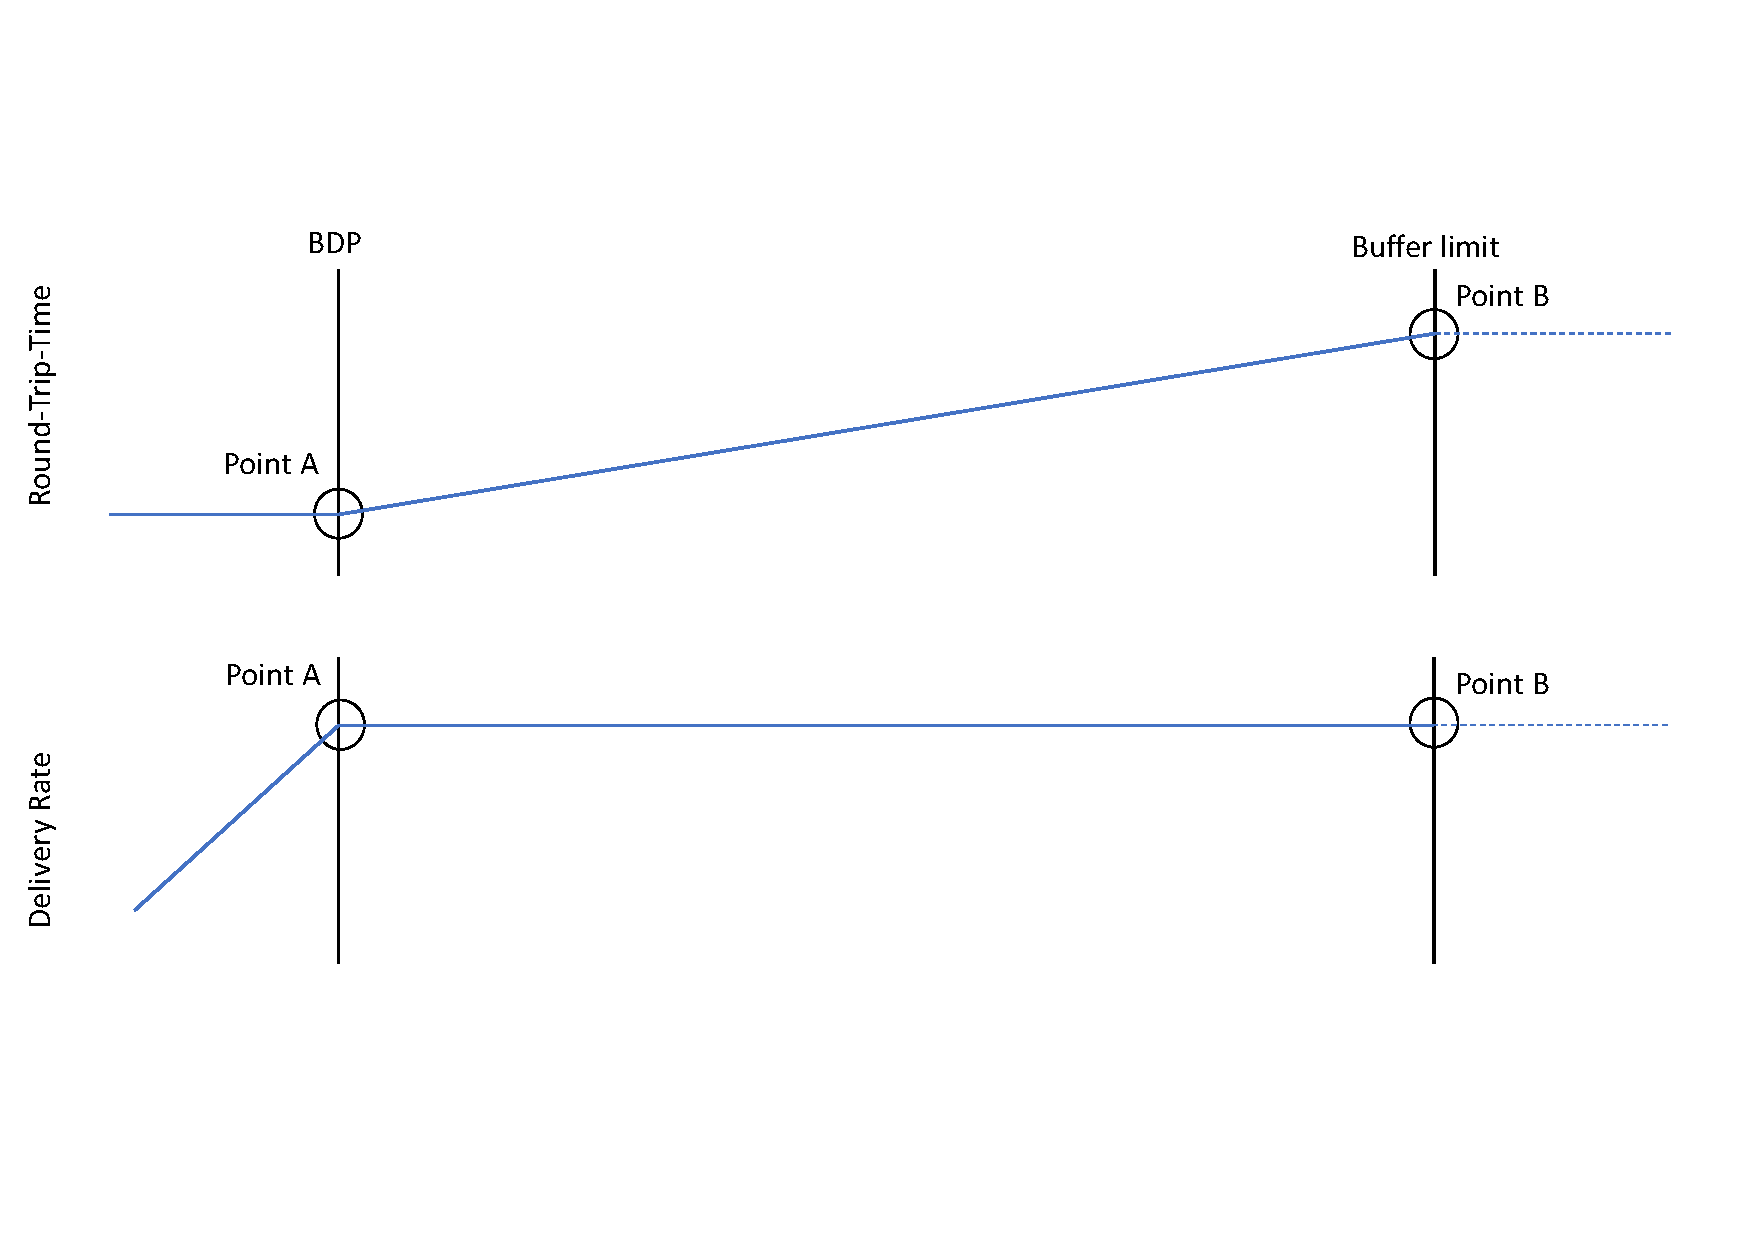
\includegraphics[width=\linewidth]{figures/ProblemForCCAs.pdf}}
\caption{Diagram that shows where different operating points for Congestion COntrol ALgorithms are. Based on \cite{BBRORIGINAL,BBREVALUATION}}
\label{ProblemForCCAS}
\end{figure}

The fundamental goal of a Congestion Control Algorithm is to maximize throughput while maintaining a low delay. 
To determine the ideal performance of such an algorithm, it is necessary to identify the optimal operating point by observing how network dynamics shift as a sender increases its transmission rate. 
As illustrated in \ref{ProblemForCCAS}, the relationship between the sending rate, the delivery rate, and the RTT can be visualized through two primary diagrams. 
The top diagram tracks the RTT, while the bottom diagram displays the delivery rate, highlighting two critical thresholds labeled Point A and Point B.  

Point A represents the moment the delivery rate equals the BDP, indicating that the bottleneck link is fully utilized.
Beyond this point, the delivery rate plateaus because the bottleneck has reached its maximum physical capacity. 
If the sender continues to increase its rate past Point A, the excess packets are forced to accumulate in the bottleneck's buffer, creating a queue. 
This accumulation causes a linear increase in RTT, as seen in the upper diagram of \ref{ProblemForCCAS}, because packets must wait longer in the queue before being processed.  
Eventually, if the rate increases further, the system reaches Point B, which signifies the buffer limit. 
At this stage, the bottleneck can no longer accept new packets, leading to packet drops and severe congestion. 

In addition to these performance metrics, another critical benchmark for evaluating a congestion control algorithm is its fairness toward other flows competing for resources at the bottleneck. 
While the behavior shown in \ref{ProblemForCCAS} suggests that the optimal operating point for an individual sender is exactly at Point A, a high-quality algorithm must also ensure an equitable distribution of bandwidth. 
To quantify this behavior, one of the most widely utilized metrics for measuring the quality of resource distribution is Jain's Fairness Index. 
Therefore, an ideal congestion control algorithm should not only target maximum efficiency but also maintain a harmonious coexistence with concurrent flows to prevent starvation or unfair resource dominance.

\subsection{BBR}

The authors of \cite{BBREVALUATION} conducted an extensive study on the performance and quality of BBR, initially testing it with multiple self-competing flows and subsequently against TCP Cubic flows. 
Their results indicate that multiple concurrent BBR flows tend to overestimate available bandwidth, which leads to persistent queue accumulation at the bottleneck. 
In scenarios involving two BBR flows, for instance, the total BDP can reach twice the actual BDP of the link.  
If the bottleneck possesses a large buffer, it may successfully handle these flows, placing the operating point somewhere between the ideal Point A and the buffer limit at Point B from \ref{ProblemForCCAS}. 
However, if the bottleneck buffer is small, BBR flows operate significantly beyond Point B, resulting in severe packet loss. 
While TCP Cubic also experiences retransmissions in these scenarios, they are significantly less frequent than those observed with BBR. 
Even when the bottleneck buffer size is set to $0.8 \times BDP$, the retransmission rate for BBR remains enormous.

Furthermore, experiments in \cite{BBREVALUATION} demonstrate that BBR faces significant challenges when competing with TCP Cubic flows. 
In large buffers, TCP Cubic tends to fill the queue, making it difficult for BBR to accurately estimate the correct RTT. 
Conversely, in small buffers, BBR suppresses TCP Cubic flows because Cubic interprets the packet loss induced by BBR as a congestion signal and drastically reduces its sending rate. 
Given the high volume of legacy systems still utilizing TCP Cubic, BBR exhibits "unfair" behavior in real-world Internet scenarios

The extensions AQDC BBR and BBR-ES focus on resolving the issue of accumulated packets in the bottleneck queue while offering intrinsic improvements to the core BBR algorithm.
The authors of AQDC BBR demonstrated that their improvements successfully decreased the RTT compared to standard BBR and achieved an 11\% improvement in Jain's Fairness Index. 
This improvement is largely attributed to the algorithm's ability to reduce tail latency by more than 25\% compared to standard BBR, which it achieves by explicitly modeling and compensating for "queue debt" incurred during probing phases. 
By quantifying the excess packets injected during the ProbeBW phase, AQDC BBR prevents the persistent buffer occupancy that typically compromises fairness.

Similar results were produced by the authors of BBR-ES, whose experiments showed that the algorithm maintained lower RTTs than BBR while preserving high link utilization. 
Unlike earlier delay-based variants, BBR-ES utilizes a trend-based transition mechanism and an "Extended State" stabilization phase to manage per-flow bandwidth and RTT evolution. 
These findings were validated in real-world scenarios by sending data to various Amazon EC2 instances in cities such as Tokyo, Singapore, and Virginia across varying throughput levels. 
Their research confirmed that BBR-ES achieves a consistently higher Jain's Fairness Index—often above 0.9—compared to both standard BBR and TCP Cubic. 
Additionally, measurements showed that BBR-ES consistently maintains top-tier link utilization, frequently exceeding 98\% in most experimental settings. 
By monitoring short-term indicators, BBR-ES effectively distinguishes between flows that heavily contribute to queue buildup and those that do not, allowing for targeted corrective actions and overall greater stability.

\subsection{PCC}

To demonstrate that PCC is a stable and effective congestion control algorithm, the authors conducted several comprehensive studies across diverse network environments. 
Their results consistently showed that PCC maintains high throughput and is significantly more resilient to random packet loss than traditional TCP variants. 
For instance, on unreliable lossy links, PCC can maintain over 95\% capacity even at a 1\% loss rate, whereas TCP CUBIC's performance collapses by more than ten times under the same conditions.\cite{PCCEVALUATION} 
This resilience stems from PCC's ability to distinguish between congestive loss and random link errors through its utility-maximizing framework.  

Beyond raw throughput, the studies highlighted PCC's superior reactivity to rapid network changes. 
In experiments where available bandwidth, RTT, and loss rates were modified every five seconds, PCC remained near the optimal sending rate throughout the duration of the test. 
In contrast, alternative algorithms like BBR or TCP CUBIC required significantly more time to converge to the optimum or failed to reach it entirely in such volatile environments. 
Furthermore, PCC proves to be remarkably efficient with limited resources, achieving 90\% throughput with a small buffer size, while TCP CUBIC requires thirteen times more buffer to reach the same level of performance\cite{PCCEVALUATION}. 

A critical component of PCC's evaluation is its behavior when sharing the network with other flows. 
Despite its "selfish" design focused on utility maximization, competing PCC flows are mathematically and empirically shown to converge to a stable and fair equilibrium. 
This includes strong RTT fairness, where flows with different propagation delays receive their fair share of bandwidth rather than the shorter-RTT flow dominating the link—a common flaw in protocols like TCP CUBIC. 
Regarding TCP friendliness, while "classic" PCC is designed to outperform legacy congestion control algorithms, the framework can be adjusted to be more "socially" compatible with traditional flows, ensuring that PCC does not completely starve existing flows traffic in mixed-protocol environments.

\subsection{Copa}

\subsubsection{Basic Copa}

The primary objective of the Copa authors was to develop a congestion control algorithm that is both high-performing and simple to understand. 
While evaluating an algorithm's "simplicity" is inherently subjective and less straightforward than quantitative metrics, several comparisons highlight Copa's relatively low complexity.  

For instance, PCC is built upon a framework that uses online learning and utility maximization, which can be complex to reason about due to its continuous "micro-experiments" of different sending rates. 
In contrast, Copa's core design centers on a single target rate equation: $\lambda = 1/(\delta d_q)$, where $d_q$ represents the measured queuing delay. 
While the derivation of this formula involves advanced modeling, the resulting algorithm remains highly comprehensible.  

Furthermore, Copa operates in two distinct modes to ensure versatility: a default mode for low-latency performance and a competitive mode designed to match the aggressiveness of buffer-filling schemes like TCP Cubic. 
The transition between these modes is determined by straightforward measurements.
The sender switches to competitive mode if it fails to detect a "nearly empty" queue within a 5-RTT window. 
While BBR also relies on limited parameters — specifically its estimates of Bottleneck's Bandwidth and RTT — PCC adopts a more data-intensive approach, continuously aggregating various packet-level events (such as loss, throughput, and latency) into a utility function to determine its sending rate.

Overall, Copa is not the most difficult algorithm to understand, particularly when compared to other modern schemes. 
We have determined that, in contrast to algorithms like PCC—which utilizes complex online optimization and randomized controlled trials—Copa relies on a more transparent, delay-based target rate formula. 
While PCC's decision-making involves aggregating multiple packet-level events into a performance utility function, Copa's logic is driven by a straightforward relationship between sending rate and queuing delay. 
Therefore, we conclude that the authors successfully reached their goal of creating a high-performing congestion control algorithm that remains simple for humans to reason about.

We will now examine the performance of Copa. 
The authors evaluated the algorithm through various experiments, comparing it directly with other prominent congestion control schemes, including PCC, BBR, and TCP Cubic. 
A central component of this evaluation is Copa's core mechanism: the target rate equation, $\lambda = 1/(\delta d_q)$.  
In one specific set of results, the authors presented Copa's performance with the competitive mode disabled. 
These findings demonstrate that in its default mode, Copa is exceptionally effective, achieving near-ideal values for both throughput and RTT estimation. 
Specifically, when operating in this mode, Copa stabilizes at a point that optimizes the trade-off between throughput and delay, effectively reaching the optimal "Point A" described in \ref{ProblemForCCAS}. 
However, the authors noted that while enabling the competitive mode allows Copa to coexist with buffer-filling flows, this transition results in significantly higher queuing delays and a deviation from these ideal performance metrics.

Furthermore, the authors conducted experiments to evaluate how their algorithm manages a varying number of flows by adding and terminating flows within an emulated network. 
They did the same for BBR, PCC and TCP Cubic.
The results indicate that Copa and TCP Cubic are most effective at maintaining ideal throughput and achieving a high Jain's fairness index, with Copa reaching a median index of 0.86 compared to TCP Cubic's 0.81. 
In contrast, BBR and PCC showed lower median fairness indices of 0.61 and 0.35, respectively. 
Moreover, the study demonstrates that Copa significantly outperforms PCC and BBR in handling changing network conditions, as it converges quickly to correct fair rates.

\subsubsection{Upgrades of Copa (Copa+ and Copa-D)}

Although Copa demonstrates strong performance, the authors of Copa+ and Copa-D identified a significant limitation: the algorithm frequently triggers its competitive mode unnecessarily. 
This premature switching leads to unintended queue accumulation at the bottleneck, compromising the low-latency benefits of its default state. 
Consequently, while Copa achieves near-optimal performance in isolation, the activation of its competitive mode often degrades its overall efficiency, even in isolation. 
To address this, extensions such as Copa+ and Copa-D introduce refined mechanisms for mode-switching logic. 
Specifically, Copa+ incorporates an additional control parameter, while Copa-D utilizes a redefined expression for $\delta$.

Copa+ utilizes this supplemental parameter to prevent erroneous transitions into competitive mode, a claim supported by the authors' experimental results. 
The algorithm consistently maintains RTT values that align with the ideal targets, effectively mirroring the performance of standard Copa when its competitive mode is disabled. 
Therefore, Copa+ successfully addresses the primary flaw of unnecessary mode switching. 
However, as the authors do not provide specific throughput statistics, a definitive conclusion regarding its impact on link utilization cannot be reached.

The authors of Copa-D evaluated their algorithm through several experiments, including scenarios where the available bandwidth was varied at fixed intervals. 
By comparing Copa with their proposed upgrade, Copa-D, they demonstrated how bandwidth fluctuations influence RTT. 
While standard Copa exhibited a highly volatile RTT, Copa-D remained relatively stable. 
This stability is expected since the experiment does not introduced delay, which therefore should ideally not trigger an RTT increase.
However, standard Copa's RTT rose with some bandwidth changes, probably due to unnecessary mode switching while Copa-D maintained a lower average RTT than the original algorithm.

It is noteworthy, however, that the experimental results indicate that Copa-D's RTT oscillates around a target value. 
Interestingly, when standard Copa stabilizes at that same point, its oscillations appear smaller than those of Copa-D. 
The authors attribute this behavior of Copa-D to the dynamic adjustment of $\delta$, which, while stabilizing the average RTT, introduces more frequent minor fluctuations.

Furthermore, the authors tested Copa-D in 4G and 5G network environments. 
Their findings reveal that while standard Copa achieves a slightly higher throughput, its RTT is significantly higher than that of Copa-D. 
This indicates that Copa-D successfully prioritizes lower delay, providing a more stable performance profile in mobile network scenarios.

In summary, Copa represents a compelling congestion control algorithm due to its inherent simplicity and robust performance. 
Through extensions such as Copa+ and Copa-D, the protocol can be tailored to operate efficiently across various specialized use cases. 
However, a significant gap remains regarding its performance in real-world network environments. 
Existing studies primarily rely on controlled experiments, leaving it unclear how effectively Copa and its variants perform outside of emulated settings.
On the public internet, flows rarely exist in isolation.
Instead, multiple heterogeneous algorithms compete for the same bottleneck resources. 
Notably, the evaluations for Copa+ and Copa-D do not adequately address scenarios where the competitive mode is essential, such as when sharing a link with aggressive, buffer-filling protocols like TCP Cubic. 
Consequently, further research is required to determine if these refinements maintain their advantages when faced with the diverse and unpredictable traffic patterns of the global internet.

\subsection{PowerTCP}

The authors of PowerTCP designed their congestion control algorithm specifically for data center networks rather than the public internet. 
This targeted approach is significant because it allows the algorithm to leverage the unique characteristics of controlled environments. 
Unlike the broader internet, a data center is typically managed by a single entity that can mandate the use of specific protocols across the entire infrastructure. 
Consequently, the authors' use of a fat-tree topology for their test environment closely reflects real-world data center network conditions. 
Furthermore, this controlled setting eliminates the need to accommodate legacy systems or outdated congestion control algorithms, which are rarely a factor in modern data center deployments.

The experimental results demonstrate that PowerTCP reacts rapidly and accurately to congestion while maintaining high throughput. 
A key performance indicator is the algorithm's ability to maintain a near-empty queue at the bottleneck, suggesting that PowerTCP operates close to the ideal operating point A described in \ref{ProblemForCCAS}. 
When additional flows are introduced, the algorithm ensures a fair distribution of bandwidth. 
Although the authors do not utilize standard fairness measures like Jain's Fairness Index for direct comparison, independent research \cite{TCPSTHIRDEYE} has successfully reproduced these findings. 
These independent studies confirm that while TCP Cubic consistently fills buffers—resulting in increased queuing delay—PowerTCP maintains minimal occupancy. 
Additionally, PowerTCP flows remain stable and equitable when sharing a bottleneck, whereas TCP Cubic flows often exhibit instability or unfair dominance.

A critical aspect of the authors' evaluation was the impact of PowerTCP on different flow durations, categorized as short, medium, and long flows. 
Their data proves that short flows receive the most significant performance benefits, while medium flows show moderate improvements. 
Long flows also perform effectively, showing no degradation in performance when compared to traditional algorithms. 
This overall efficiency is primarily driven by INT, which provides PowerTCP with a comprehensive real-time view of the network status.

In summary, PowerTCP is highly effective within its specialized niche. 
It successfully achieves high throughput with minimal delay by preventing queue buildup. 
However, its heavy reliance on INT represents a significant limitation.
It is highly improbable that routers or switches in the wide-area internet would provide the necessary telemetry data that the algorithm requires. 
Therefore, while PowerTCP is an optimal choice for congestion control within a data center, it lacks a viable use case in general networking environments where telemetry requirements cannot be met.

\subsection{C4}

The authors of the C4 algorithm primarily focused on optimizing network flows for real-time media, such as video and audio streams, which are highly sensitive to latency and queuing delays. 
In their findings published in the C4 repository, the algorithm was rigorously compared against BBR and TCP Cubic within various simulated WiFi network environments. 
These evaluations encompassed scenarios such as WiFi suspension, fading, and extreme jitter to determine C4's robustness relative to its peers. 
In high-bandwidth basic tests, C4 and Cubic performed identically with minimal delay, whereas BBR's pacing logic resulted in a maximum audio queuing delay of significant higher than the delay observed for C4. 
Under low-bandwidth conditions (10 Mbps), C4 demonstrated a superior ability to manage high-definition video, maintaining a maximum delay than that from BBR. 
Furthermore, during extreme jitter tests, C4 utilized tighter transmission control by pacing traffic at approximately 29 Mbps for a 20 Mbps link while BBR is pacing at 58 Mbps, which successfully prevented video spikes from interfering with high-priority audio traffic. 
Even in challenging suspension scenarios, C4 proved to be more efficient than TCP Cubic and neared the performance levels of BBR, illustrating its effectiveness as a modern congestion control solution for media-heavy applications.

In summary, current evaluations of C4 are limited by a lack of performance data regarding its behavior in network environments beyond Wi-Fi. 
Furthermore, there is an absence of empirical evidence concerning its fairness when competing with other flows or just multiple flows of its own, as the provided datasets do not address how C4 interacts with diverse traffic types. 
Given its demonstrated advantages over TCP Cubic and BBR in wireless scenarios—particularly in reducing queuing delay for real-time media—C4 warrants further testing in varied network architectures to determine if its effectiveness persists across different environments. 
Additionally, a significant research gap exists because there is no direct comparison between C4 and the Copa algorithm or its extensions. 
While existing data suggests that Copa might offer competitive performance, a definitive conclusion cannot be reached because the respective tests were conducted in disparate network conditions, making a direct side-by-side evaluation impossible at this time.
